\chapter{Introduction}
% The upper atmosphere of the earth (90 km+, defined in section \ref{sec:str}) is influenced by forcing from below (the lower atmosphere) as well as forcing from above (the sun). The upper atmosphere is in a weak plasma state due to ionization of chemical species by high energy solar radiation. Understanding the processes in the upper atmosphere thus is important. In this thesis, we study the upper atmosphere during two phenomenon: one involving particle entry and the other involving dynamics generated by thermal changes.
\section{Dissertation Outline}

This thesis is focused on observing the Thermosphere-Ionosphere (TI) system, which lies in the earth's upper atmosphere, using a ground-based multi-spectral imager known as High Throughput \& Multi Slit imaging Spectrometer (HiT\&MIS). Based on observations, two different phenomenon are studied. The first phenomena involves estimation of the energitics of solar particle entry during an auroral event. The second phenomena involves temperature changes in the upper atmosphere that leads to waves. In this chapter, first, background on the earth's atmosphere and the TI system is given; then, information on how the observation is tied to the TI system is provided. In chapter 2, details on different instruments that were used for this thesis is provided. Chapter 3 describes methods created to simultaneously derive the energy and flux of electrons penetrating into the atmosphere based on multi-spectral imaging of auroras. Chapter 4 presents characterization of Traveling Ionospheric Disturbances (TIDs) generated by Atmospheric Gravity Wave (AGWs) observed using multiple instruments including HiT\&MIS.

This dissertation contains modified versions of the publications "Derivation of the energy and flux morphology in an aurora observed at mid‐latitude using multi‐spectral imaging"  by \citep{aryal} and "Multi-spectral and multi-instrument observation of TIDs following the Total Solar Eclipse of August 21, 2017" by Aryal et al b. [in review].


\section{Structure of the Atmosphere}
\label{sec:str}
Earth’s atmosphere can be divided into many different layers based on the temperature profile, how the chemical species mix and the differences in dominant physical processes and so on. In terms of the temperature profile, the Earth’s atmosphere is divided into: 
\begin{itemize}
	\item The troposphere (0 -15 km in altitude), where temperature decreases with altitude due to decrease in infrared radiation from the Earth. 
	\item The stratosphere (15-50 km), where there is an increase in temperature as UV radiation is absorbed by ozone, the mesosphere (50-90 km) where the temperature decreases due to radiative cooling.
	\item The thermosphere (90-600 km), where the temperature increases rapidly due to absorption of high energy solar radiation.  High energy solar radiation also ionize chemical (neutral) species in the thermosphere creating the ionosphere.
\end{itemize}
In terms of mixing, the Earth’s atmosphere is divided into two regions. 
\begin{itemize}
	\item The heterosphere (up to 100 km) is where all the chemical species are well-mixed due to turbulence. 
	\item The homosphere ($>$ 100 km) is where chemical species are not well-mixed due to diffusion and the density structure of each species is determined by mass. That is, the lighter chemical species are found higher in the atmosphere.  
\end{itemize}
In terms of differences in dominant physical processes, the Earth’s atmosphere is divided into 
\begin{itemize}
	\item the lower atmosphere (0-15 km), 
	\item the middle atmosphere (15-90 km) and 
	\item the upper atmosphere (90 km and above). 
\end{itemize}

\begin{figure}[t]
	\centering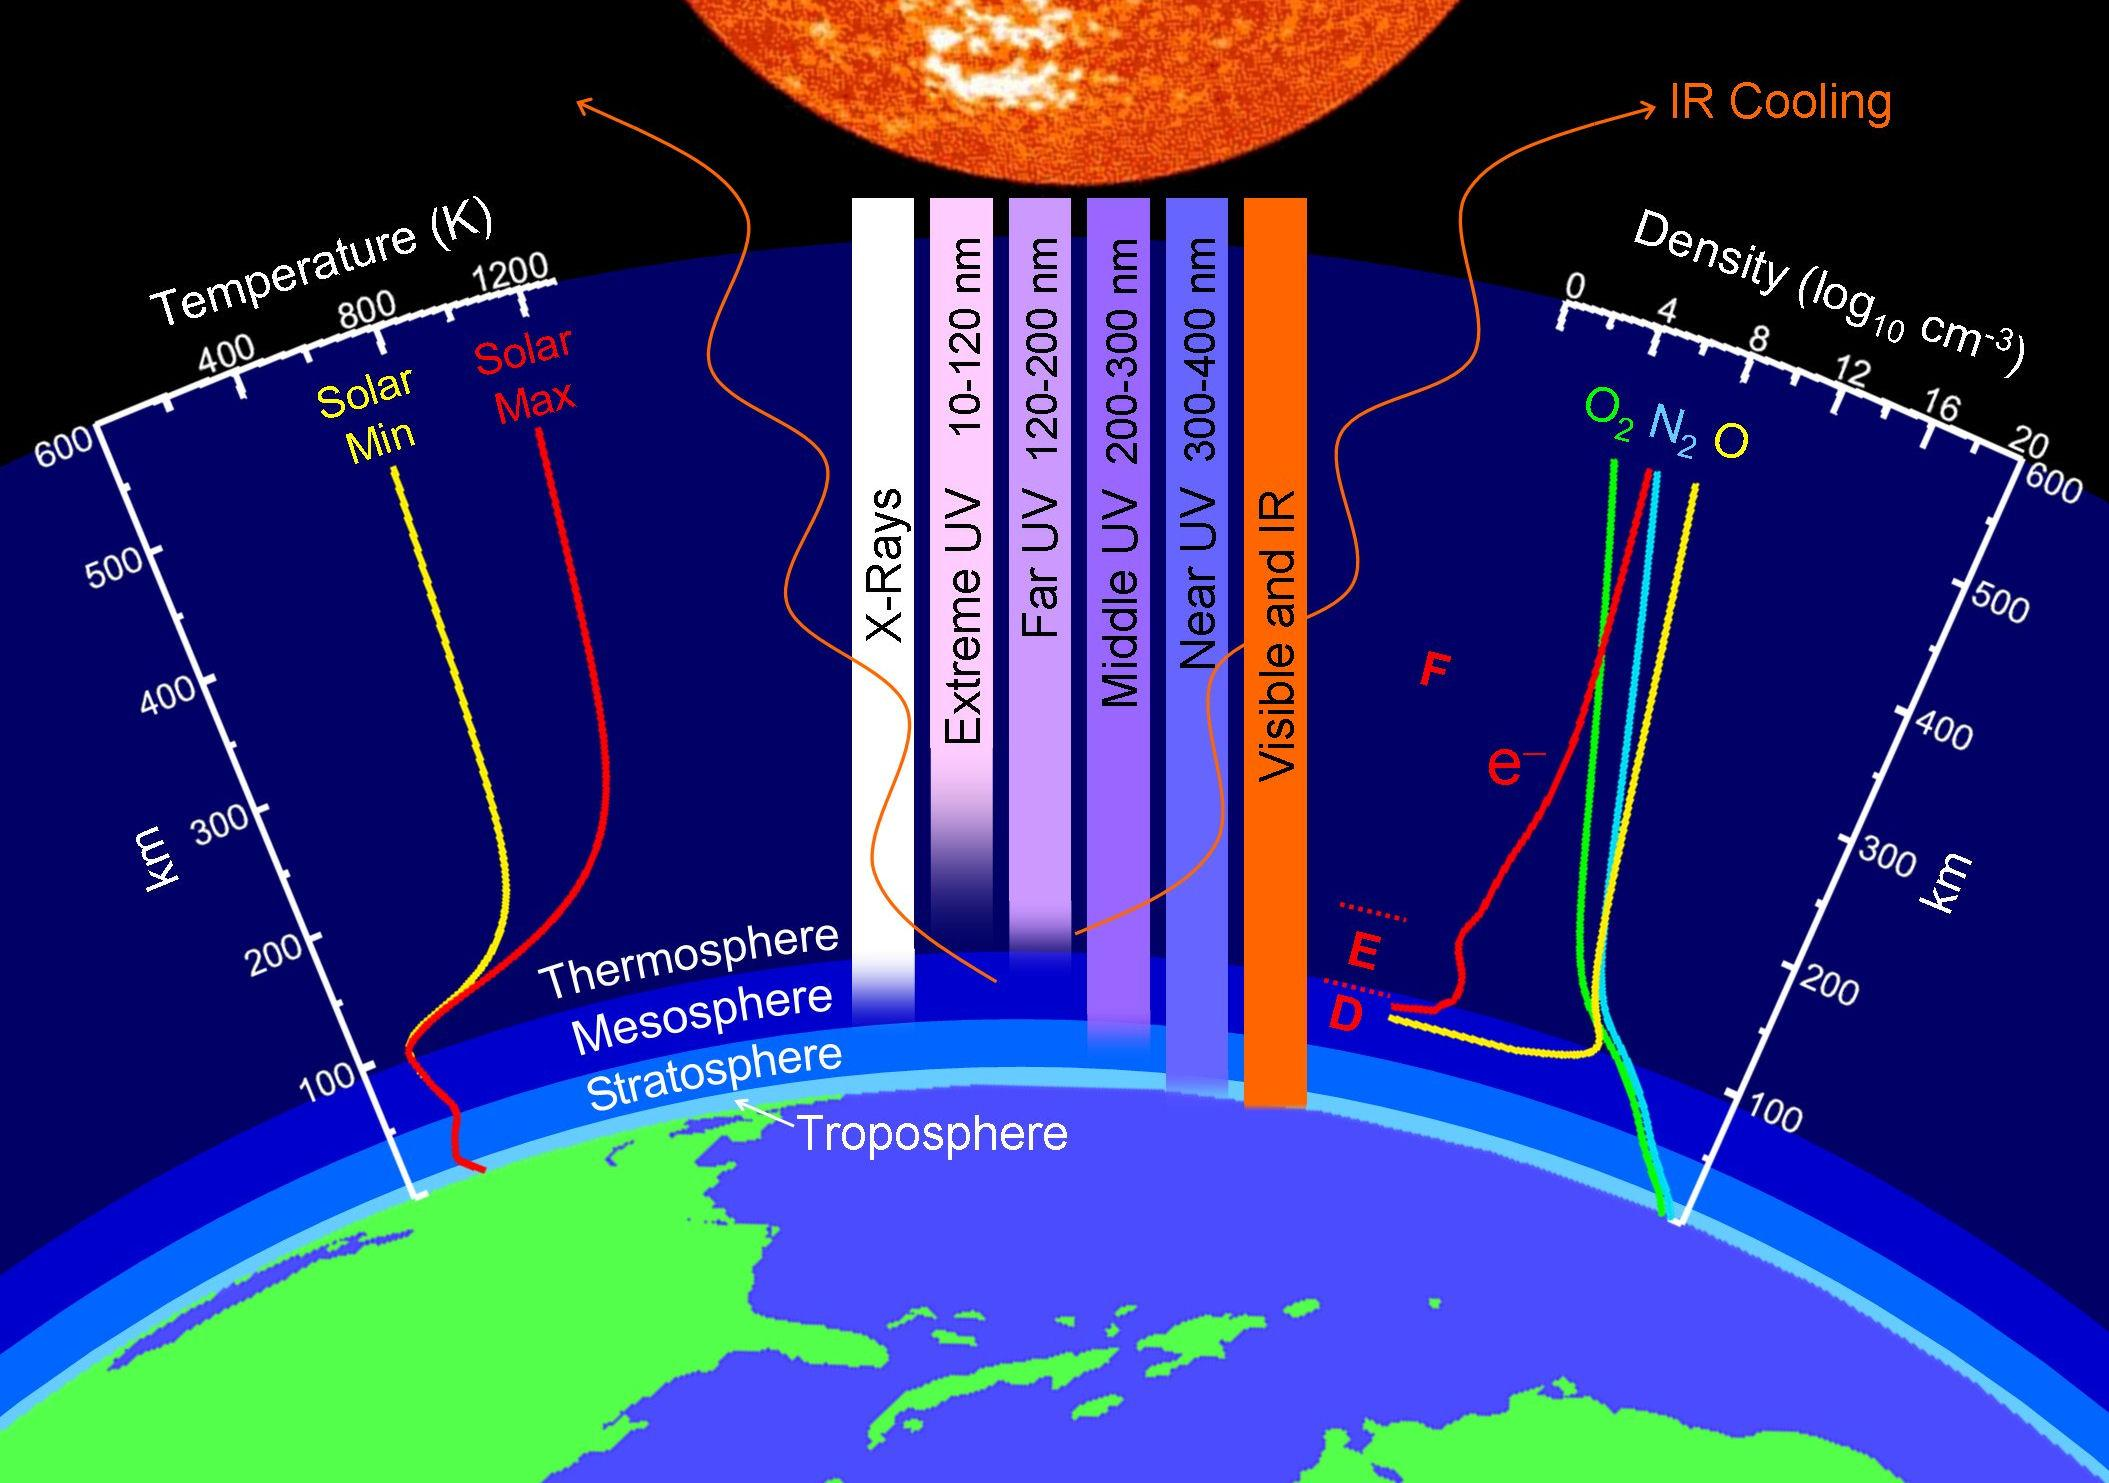
\includegraphics[width=32pc]{vert_stu.jpg}
	\caption{Vertical structure of the Earth's atmosphere in terms of temperature, density of chemical species and where solar radiation at different wavelengths get absorbed. Source: John Emmert, NRL}
	\label{fig:vert_str}
\end{figure}

%%%%


\section{Theory of the Planetary Atmosphere}
In 1D geometry (put a simple figure) the pressure (p) gradient can be written as:
\begin{equation}
\label{eq:he}
\frac{dp}{dz} = -g(z) \rho
\end{equation}
which comes from applying Newton's second law to small parcel of gas with density ~$\rho$ contained in height, dz. Assuming ideal gas, we can write the pressure (p) as $\frac{\rho}{M}$ k T, where k is the Boltzmann's constant, T is the temperature, and M is the molecular mass of the gas. Replacing the pressure (p), and assuming p and T not function of height (z), equation \ref{eq:he} becomes:
\begin{equation*}
\frac{dp}{dz}= -p \frac{M g}{k T} = -\frac{p}{H}  \\
\end{equation*}
\begin{equation*}
\implies \frac{dp}{p}=-\frac{dz}{H}
\end{equation*}
\begin{equation}
\label{eq:p}
\implies p (z)= p(z_{0}) e^{-\frac{z-z_{0}}{H}} \implies n(z)= n(z_{0}) e^{-\frac{z-z_{0}}{H}} 
\end{equation}
where, H = $\frac{k T}{M g}$ is known as the scale height, z$_0$ is the reference height and n is the number density. The scale height, H, is the height at which the pressure (and the number density) drops by $\frac{1}{e}$.  For the heterosphere, i.e. the well mixed atmosphere < 100 km, M is the mean molecular weight of all the atmospheric species. Above $\rm \sim$100 km (homosphere), the chemical species diffusively separate and each chemical species follow their own scale height, H$_i$= $\rm \frac{k T}{M_{i} g}$ ; where H$_i$ and M$_i$ are the scale height and the molecular mass of the i$^{\rm th}$ atmospheric species.

So far we have assumed that the temperature and the gravity are constant with respect to the atmospheric height. This is an ideal over-simplification, the gravity drops smoothly with height and the temperature changes differently at different layers of the atmosphere (see Section \ref{str}). There are also various chemical and physical processes that transport atmospheric constituents and break hydrostatic equilibrium. Thus, in general the atmosphere is sliced into thin layers where T and g are assumed to be constant. 
\begin{figure}[t]
	\centering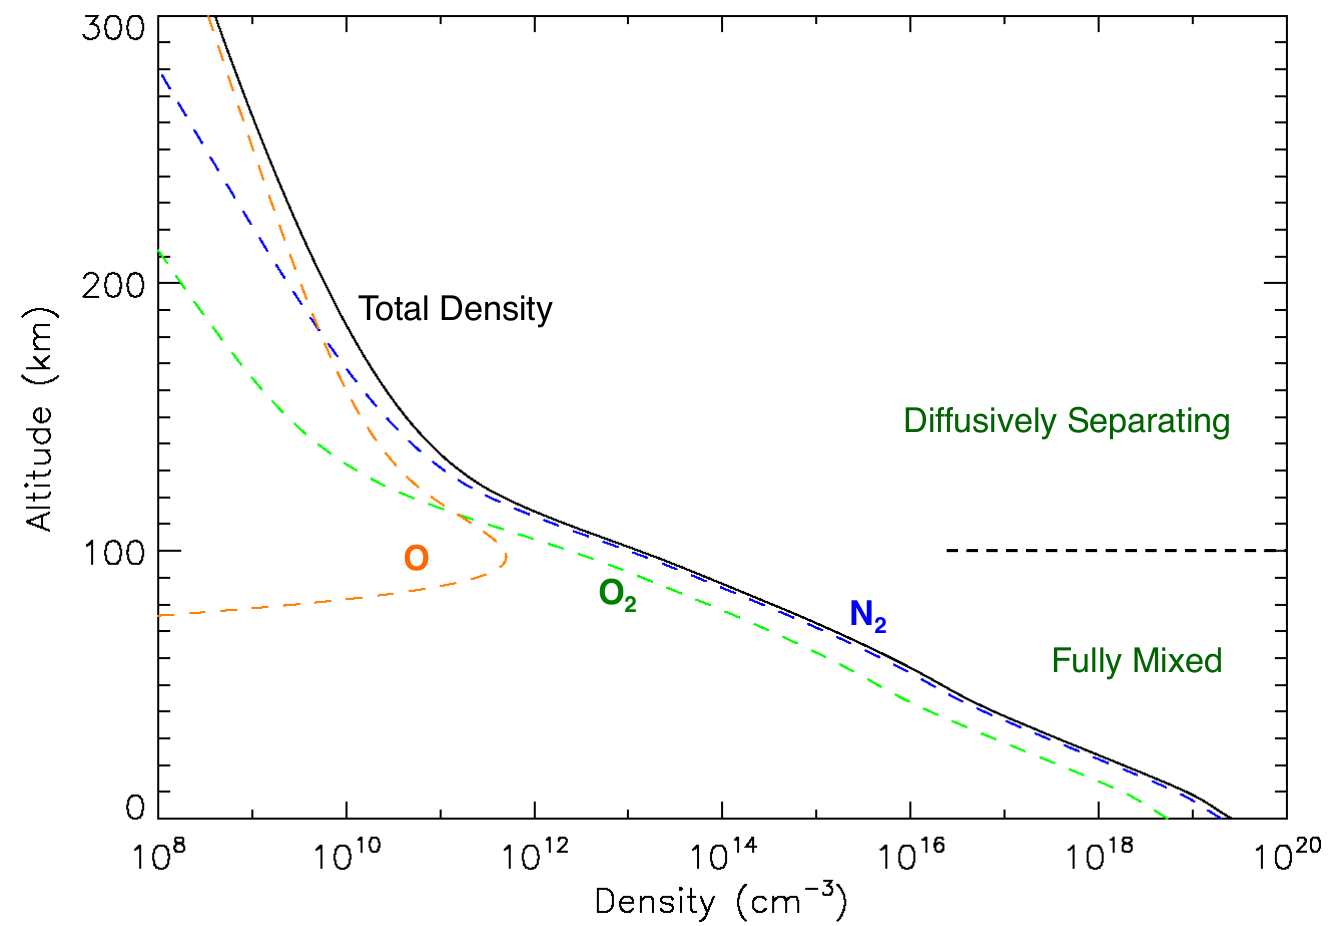
\includegraphics[width=35pc]{ok_dens_str_neu.png}
	\caption{Neutral density structure of the Earth's atmosphere. Plot courtesy Dr. Stan Solomon, NCAR}
	\label{fig:neu_den}
\end{figure}
\section{Upper Atmosphere}
The upper atmosphere is the first to receive the radiative energy input (dominant in mid and low latitudes) and in the form of charged particle input (dominant in higher latitudes) from the Sun. The high energy solar radiation (X-rays and UV) have an ionizing effect on the constituents present in the upper atmosphere, thus creating the ionosphere, the ionized part of the upper atmosphere. This the upper atmosphere is a mixture of neutral, ionized chemical species and electrons whose interactions are then affected by the presence of the Earth’s magnetic field. This thesis is focused on the remote sensing of the upper-atmosphere and specifically the thermosphere and the ionosphere (embedded within the thermosphere).

\section{Thermosphere and Ionosphere}

The upper-atmosphere is the first to receive energy inputs from the sun in form of radiation and energetic particles. In the mean time, the density of neutral gases decrease exponentially with altitude and such that the density is space-like. The high energy solar inputs and low neutral density gives rise to a favorable environment in ionizing the atoms and molecules (also dissociate molecules) creating a space like plasma environment. Furthermore, absorption of high energy solar radiation leads to heating and the temperature rises rapidly with altitude and then plateaus creating the thermosphere. Together with the charged portion of the upper atmosphere, i.e. the ionosphere, this part of the upper atmosphere is known as the Thermosphere-Ionosphere (TI).
%%%Solar spectrum
\begin{figure}[t]
	\centering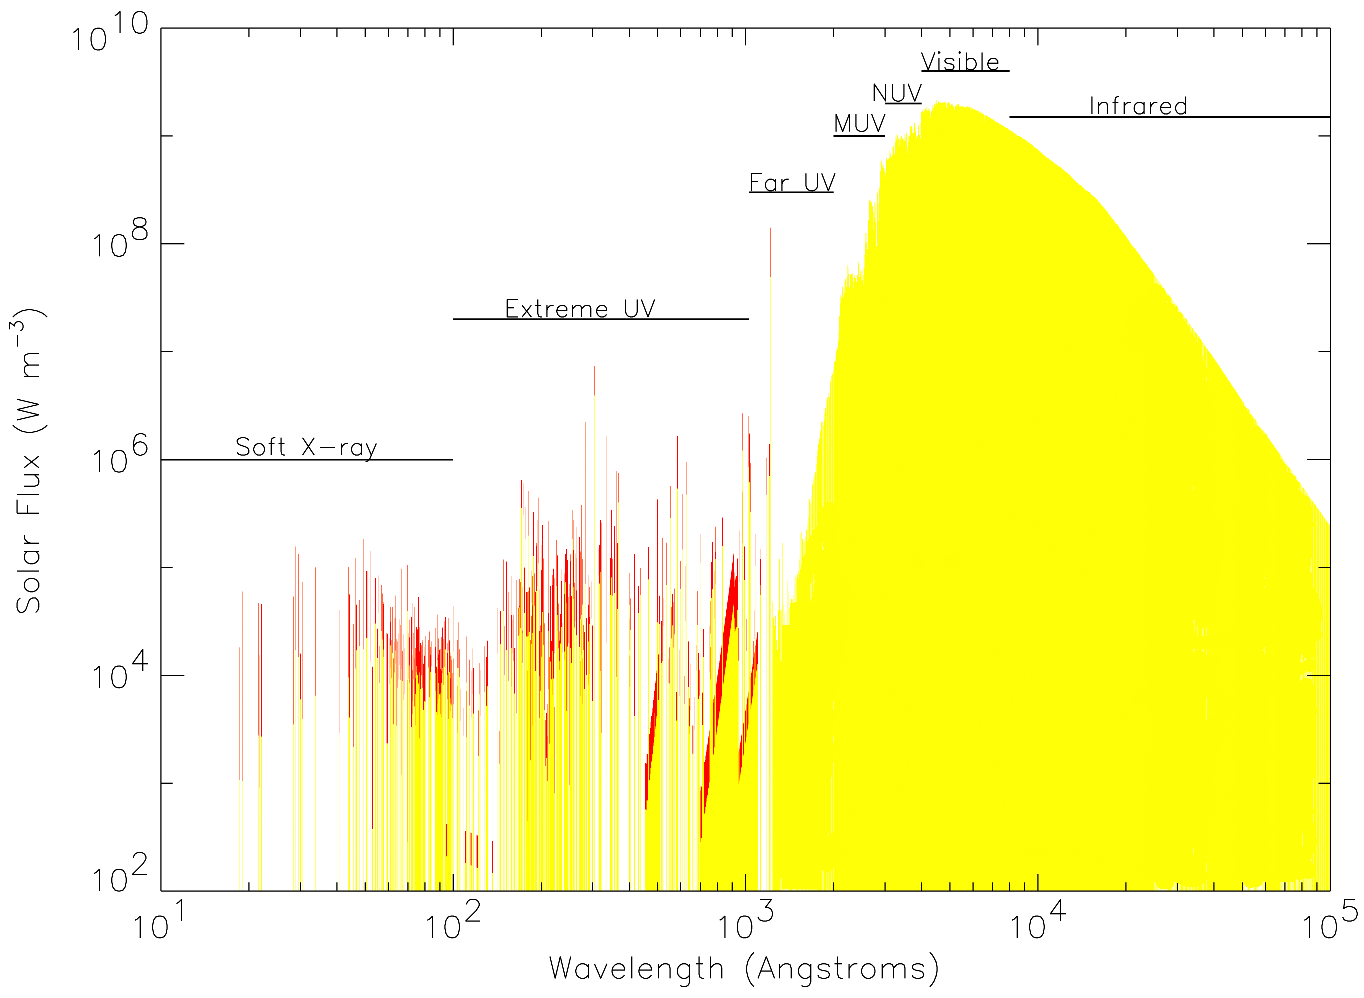
\includegraphics[width=35pc]{solar_spec.png}
	\caption{Typical example of solar spectrum incident on top of the Earth's atmosphere. Notice that the high energy radiation (X-ray and UV) vary a lot while the visible and infrared spectrum do not change. Plot courtesy of Dr. Stan Solomon, NCAR }
	\label{fig:solar_spec}
\end{figure}
%%%%%% Absorbtion of solar radiation
\begin{figure}[t]
	\centering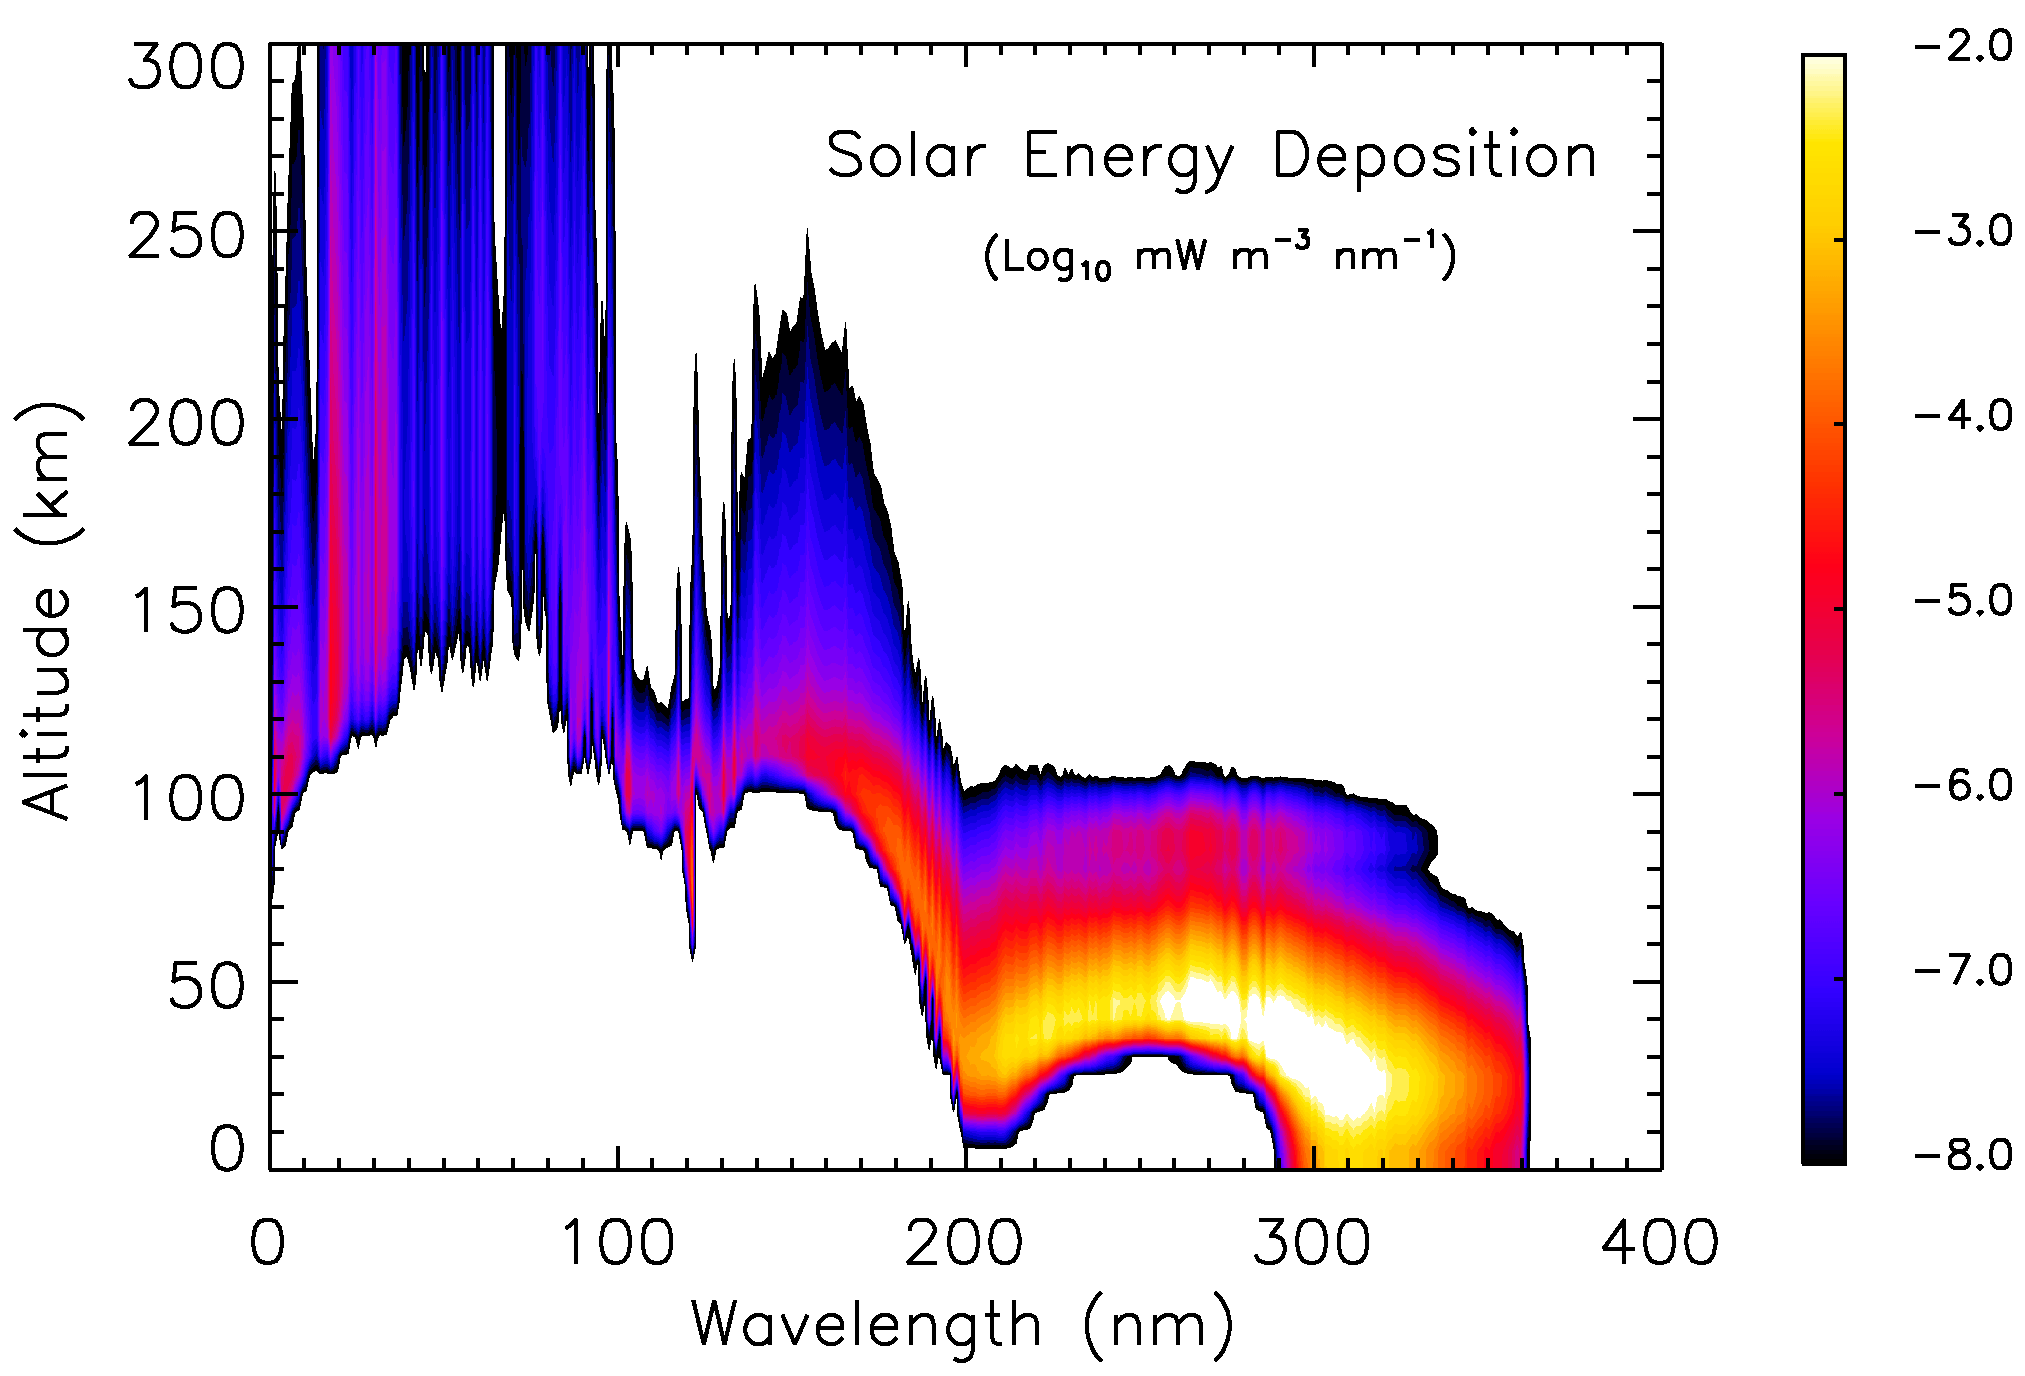
\includegraphics[width=35pc]{slr_rd_abs.png}
	\caption{Solar energy deposition in the Earth's atmosphere. Notice that most the highest energy radiation (< 200 nm) are absorbed before thy reach 100 km. Plot courtesy of Dr. Stan Solomon, NCAR }
	\label{fig:sl_rad_abs}
\end{figure}
%%%%temperature structure plot
\begin{figure}[t]
	\centering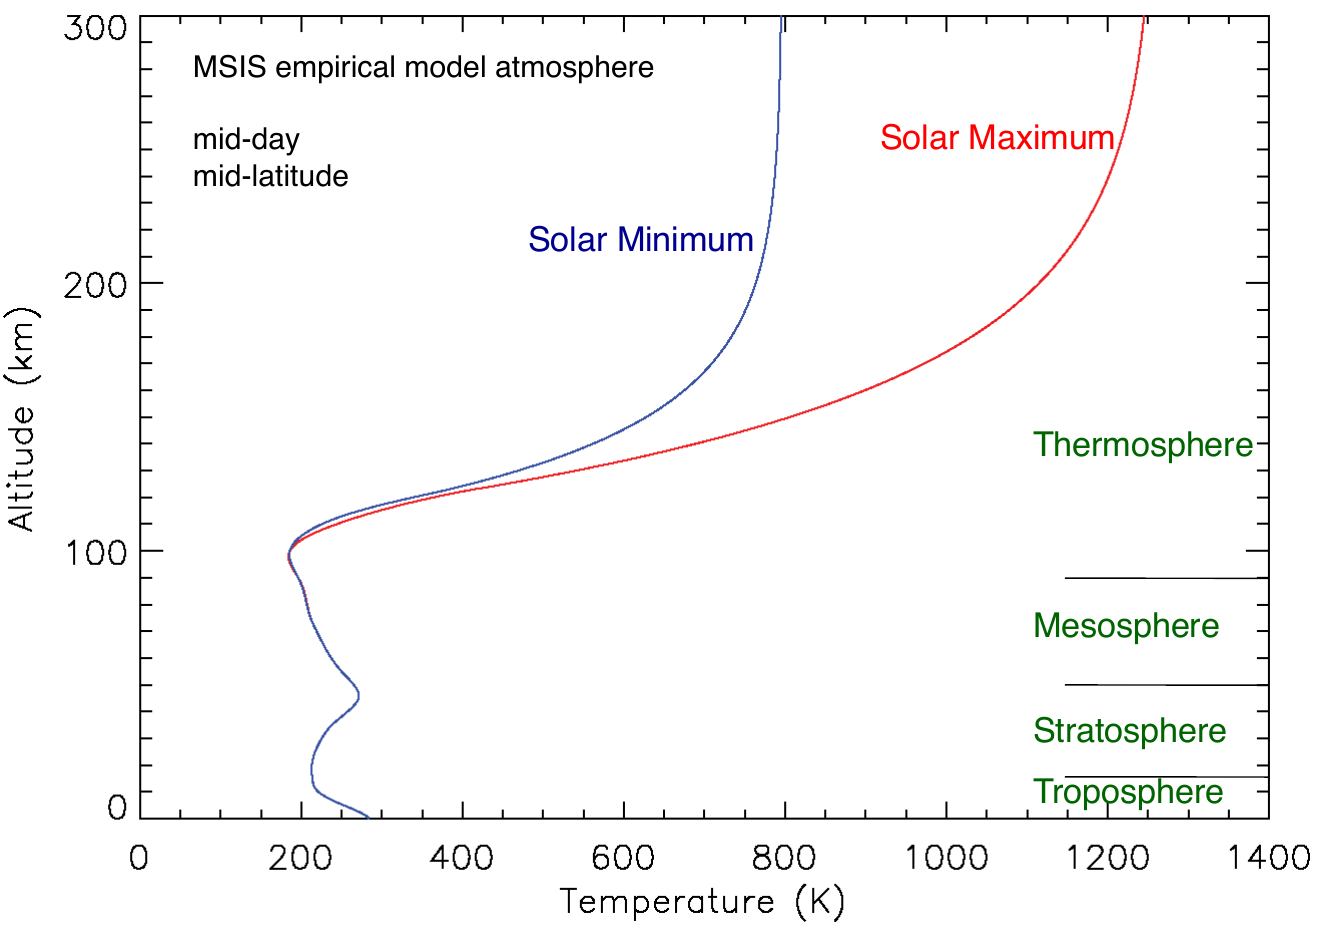
\includegraphics[width=35pc]{okl_temp_stru_slr_min_max.png}
	\caption{Temperature structure of the Earth's atmosphere based on MSIS. Notice sharp rise in temperature at the bottom of the Thermosphere which plateaus. Plot courtesy of Dr. Stan Solomon, NCAR }
	\label{fig:TI_temp_var}
\end{figure}
\begin{figure}[t]
	\centering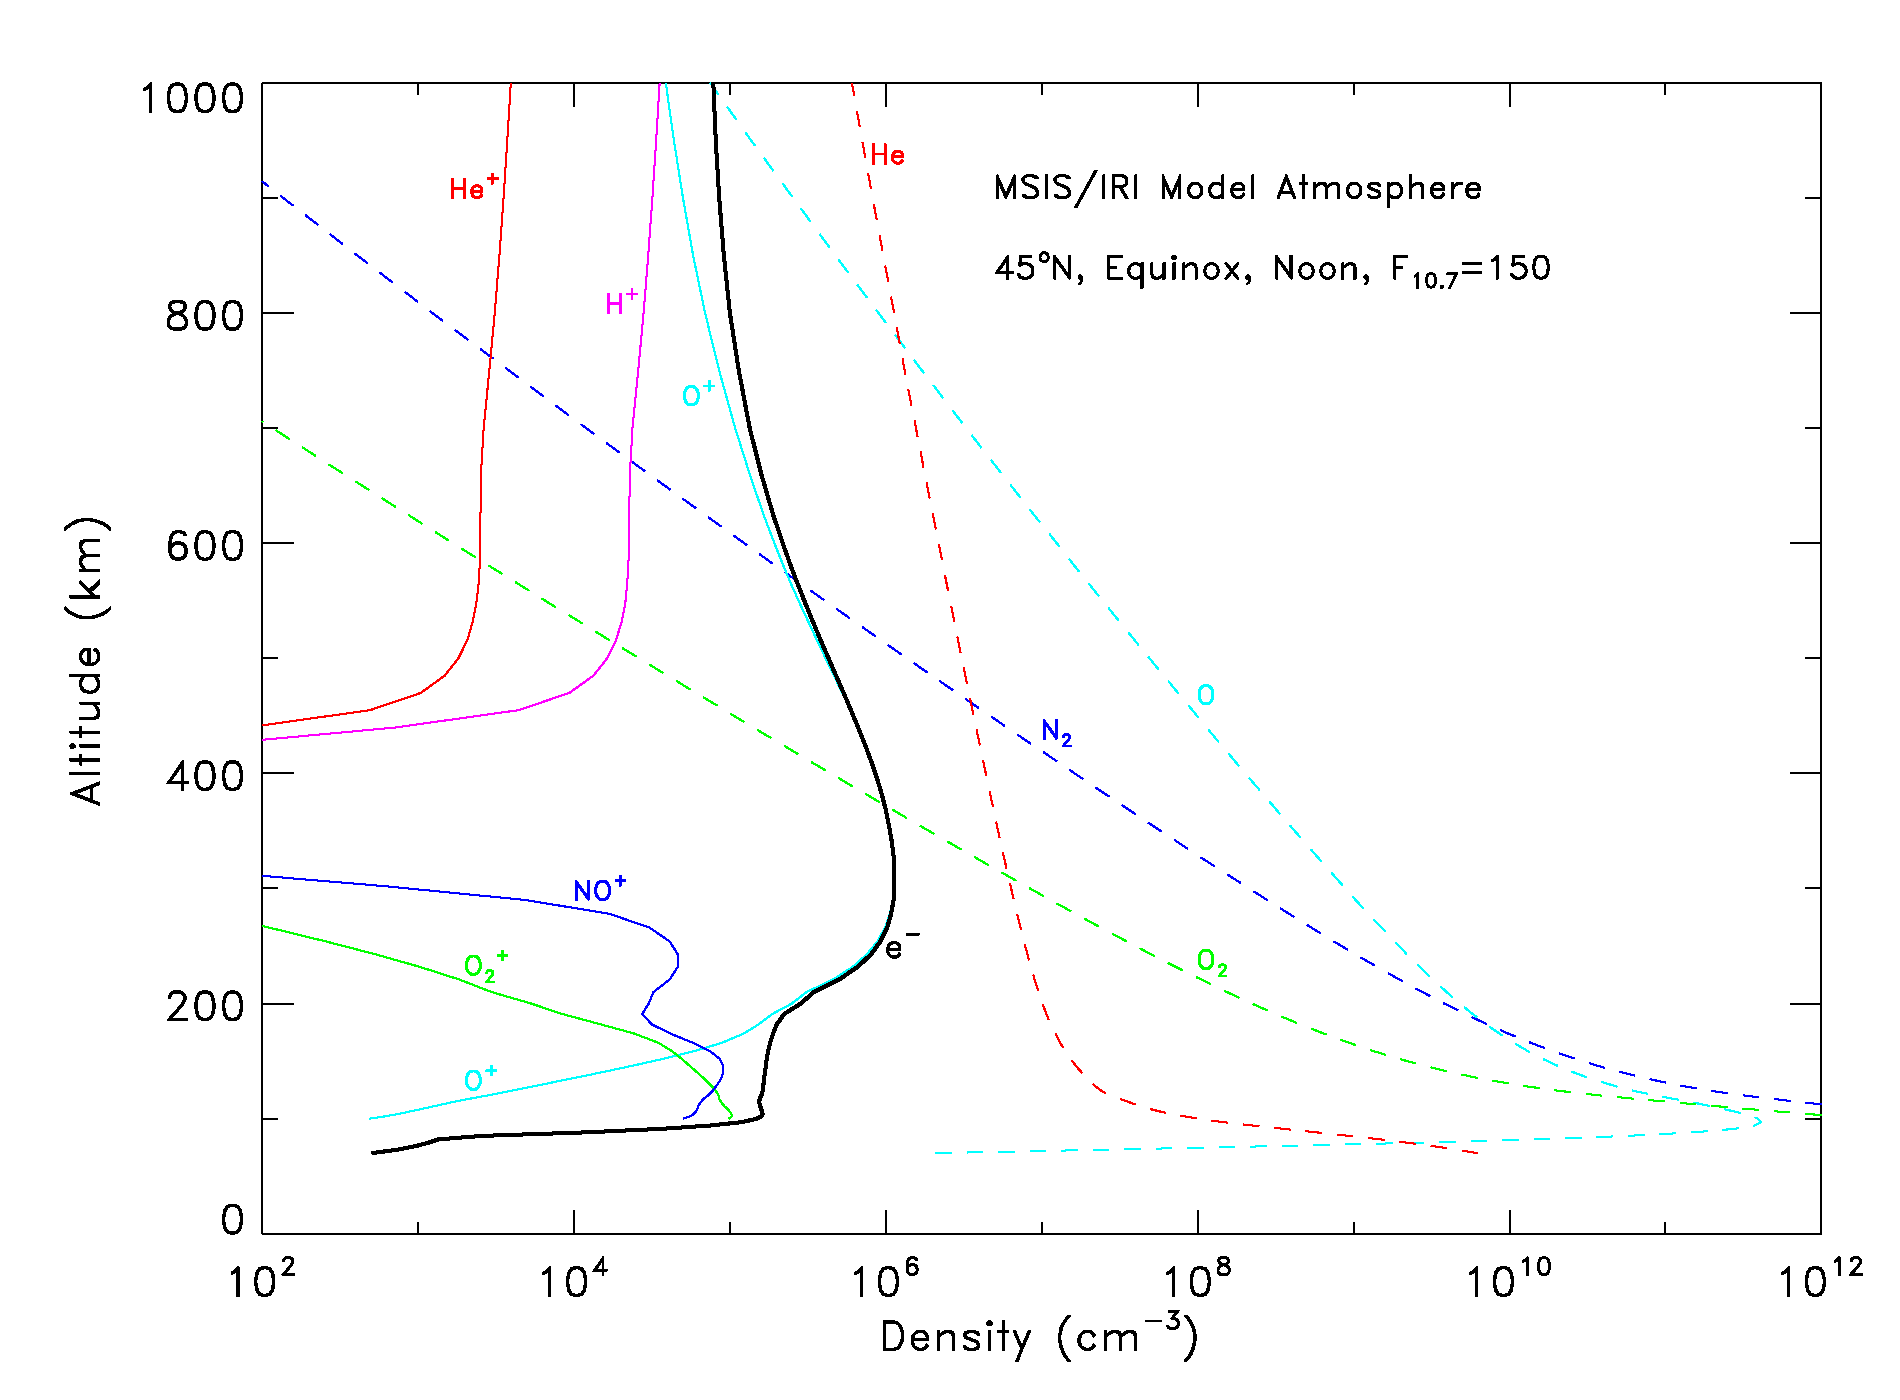
\includegraphics[width=35pc]{thm_dens.png}
	\caption{Density structure of neutral and ionic species in the Earth's atmosphere based on MSIS and IRI climatological models. Notice lighter atoms and ions are only present above $\rm \sim$ 100 km. Plot courtesy of Dr. Stan Solomon, NCAR }
	\label{fig:TI_dens}
\end{figure}
In the lower portions of the TI, the density of the neural species are high enough to get affected by the neutral dynamics (weather) at lower altitudes. Hence, the TI system is influenced by forcing from above (sun) and below (tropospheric weather). This making it an ideal laboratory to study the solar-terrestrial interaction.
\subsection{Ionosphere}
Ionization due to high energy solar radiation plus collisional ionization by energetic particles of the upper atmospheric constituents creates a weakly ionized region known as the ionosphere (about 80-1000 km).

\subsection{TI climatological Variability}
The climatological variability in the TI system is driven by the Solar Cycle. The solar cycle is the ... (put a image of solar cycle)
\begin{figure}[t]
	\centering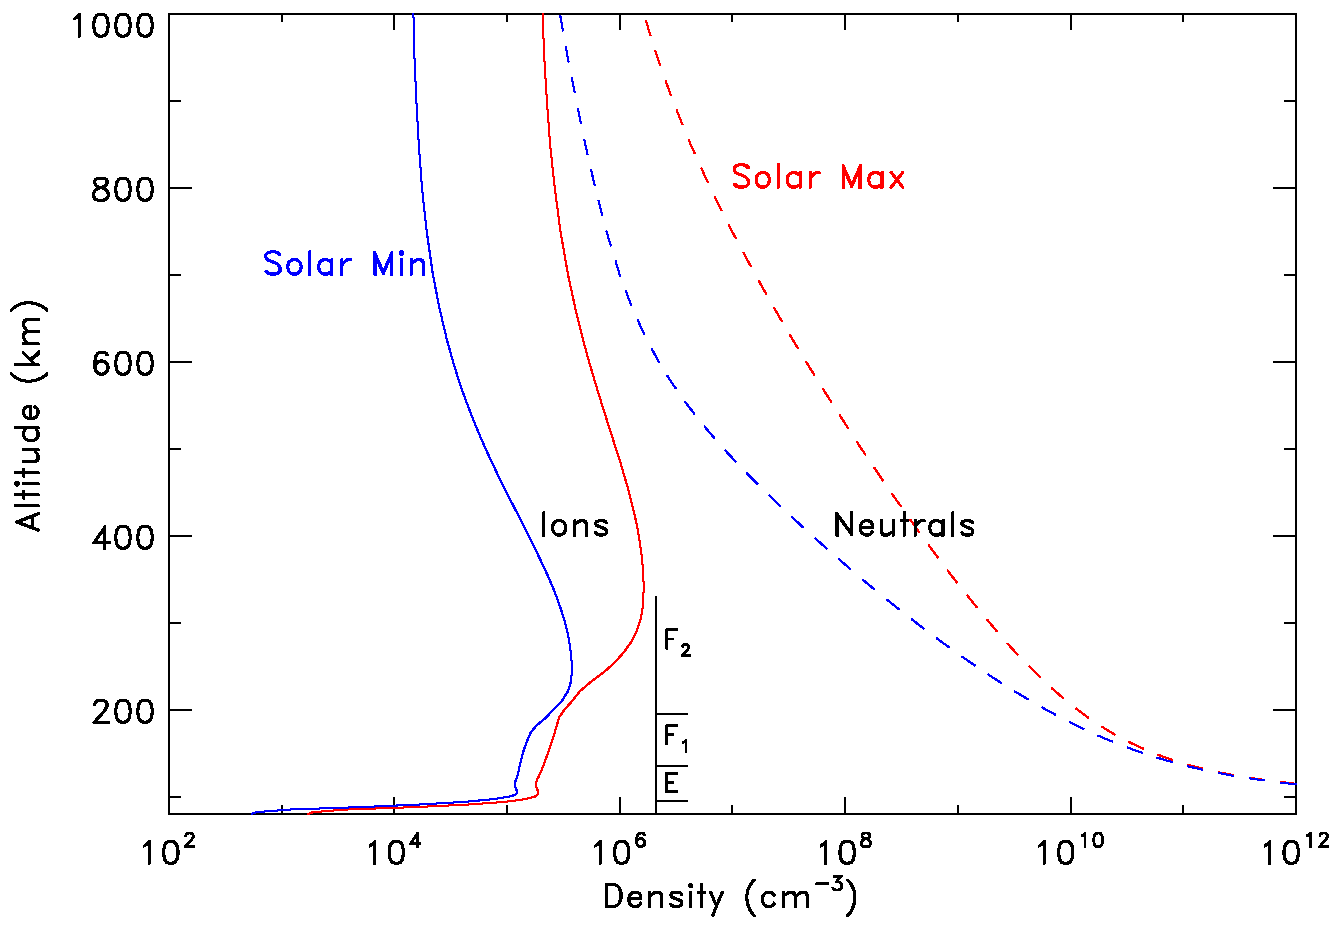
\includegraphics[width=35pc]{slr_minmax_slm.png}
	\caption{Density structure in the TI. Both ion and neutral density increase during the solar max period. Plot courtesy of Dr. Stan Solomon, NCAR }
	\label{fig:TI density variability}
\end{figure}


Thermosphere is also where most of the satellites, including the International Space Station (ISS) reside. So, studying the upper atmosphere also helps in quantifying the effects of upper-atmospheric weather (referred as space weather hereafter) on expensive satellites as well as health effects on Astronauts. In addition, different technologies based on satellites (GPS, satellite internet, etc.) could get disrupted by space weather. Like terrestrial weather, the long term goal for space weather is to predict adverse weather before hand to limit economic damage caused by such events.

\subsection{Solar inputs on the TI system}
The continuous stream of charged particles from the Sun (solar wind) with its embedded magnetic field, known as the Interplanetary Magnetic Field (IMF), hits the Earth and pushes and distorts the Earth’s magnetic field. This creates a long cigar-shaped region where charged particle motion is controlled by Earth’s magnetic field called the magnetosphere (see Fig. 1). Most of the energetic particles carried by the solar wind flow around this distorted magnetic field, except around the magnetic poles. Around the magnetic poles, the more perpendicular orientation of the Earth’s magnetic field allows more solar particles to enter the upper atmosphere of the Earth, either directly through the magnetic cusp (Fig. 1) or due to magnetic reconnection. In addition, there is a reservoir of trapped high energy charged particles around the Earth in regions known as the radiation belts (Fig. 1). These radiation-belt particles can diffuse or get accelerated into the upper atmosphere and interact with the upper atmosphere. Most of the entry of the energetic particles occurs at high latitudes; however, during solar storms (characterized by a sudden increase in speed and density of solar wind particles) particle precipitation can occur even at low and middle latitudes, but this depends on the strength of the storm and the orientation of IMF [3]. 

  

\section{Magnetosphere} 
The continuous stream of charged particles from the Sun (solar wind) with its embedded magnetic field, known as the Interplanetary Magnetic Field (IMF), hits the Earth and pushes and distorts the Earth’s magnetic field. This creates a long cigar-shaped region where charged particle motion is controlled by Earth’s magnetic field called the magnetosphere (see Fig. 1). 
\begin{figure}[t]
	\centering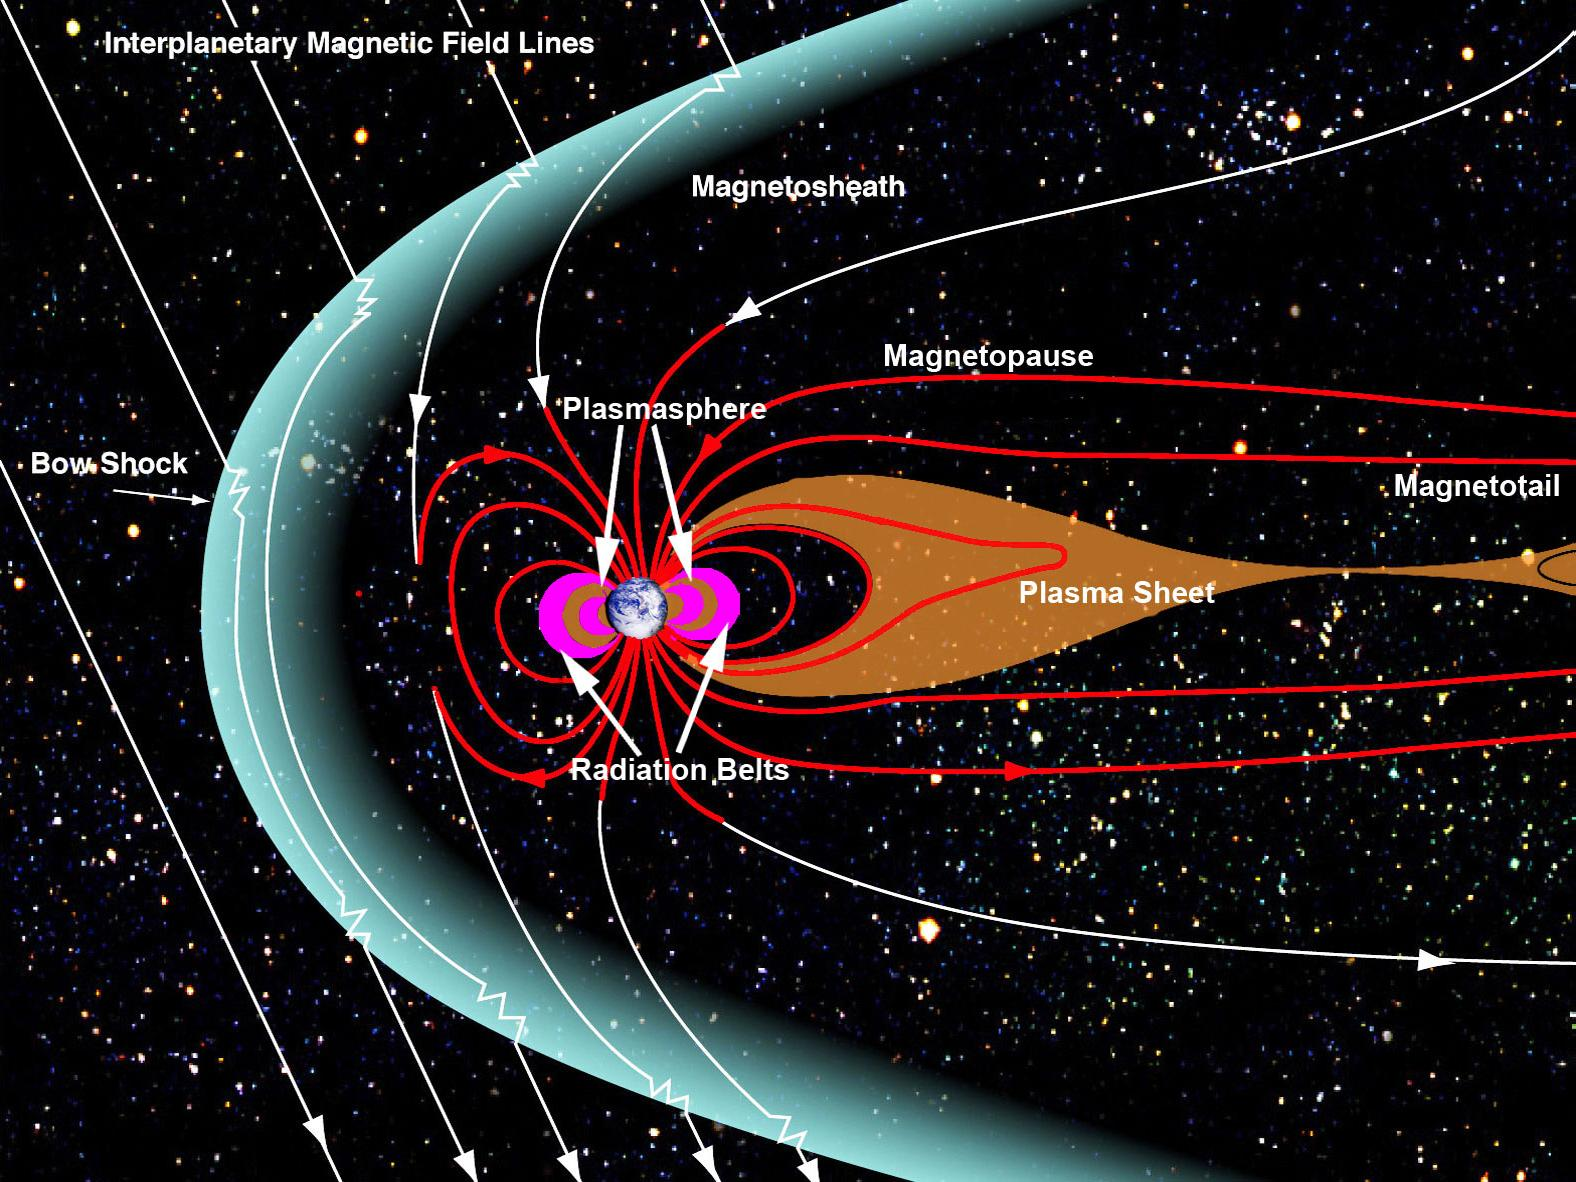
\includegraphics[width=32pc]{magne.jpg}
	\caption{Magnetosphere of the earth. Source: Aaron Kaase,NASA Goddard}
	\label{fig:magnetosphere}
\end{figure}


\section{Emissions in TI system}
Most of the energetic particles carried by the solar wind flow around this distorted magnetic field, except around the magnetic poles. Around the magnetic poles, the more perpendicular orientation of the Earth’s magnetic field allows more solar particles to enter the upper atmosphere of the Earth, either directly through the magnetic cusp (Fig. 1) or due to magnetic reconnection. In addition, there is a reservoir of trapped high energy charged particles around the Earth in regions known as the radiation belts (Fig. 1). These radiation-belt particles can diffuse or get accelerated into the upper atmosphere and interact with the upper atmosphere. Most of the entry of the energetic particles occurs at high latitudes; however, during solar storms (characterized by a sudden increase in speed and density of solar wind particles) particle precipitation can occur even at low and middle latitudes, but this depends on the strength of the storm and the orientation of IMF [3]. 
\begin{itemize}
  \item Photoionization due to high energy solar radiation plus collisional ionization by energetic particles of the upper atmospheric constituents creates a weakly ionized region known as the ionosphere (about 80-1000 km). The interaction of the electrons, called the photoelectrons or secondary electrons, depending on the process, with the neutral and ionized chemical species via collision and/or chemical processes gives rise to upper atmospheric optical emission. In general, we can categorize the optical phenomena in the upper atmosphere into two mechanisms: 

	\item  Collisional excitation due to impact of energetic charged particles generally gives rise to the aurora. These energetic particles can collisionally ionize various atomic and molecular species creating secondary electrons with different kinetic energies. These secondary electrons then change the states of the atmospheric constituents by collision and produce optical emission: line emission in the case of atoms (or atomic ions) and band emission in the case of molecules (or molecular ions). 
\end{itemize}

Photoionization, photoelectron excitation, photodissociation and other processes driven by solar radiation generally gives rise to the airglow. During the day, the solar radiation ionizes the atmospheric constituents in the upper atmosphere creating photoelectrons and dissociates molecules creating chemical species in various excited states. The photoelectrons generated by photoionization also collisionally excite chemical species into different states. During the night, the residual electrons can generate optical emission by recombination with ions. In addition, various chemical reactions in the upper atmosphere can also produce atomic (and molecular) emission. 
% put a table of main types of photochemical reactions
The six emission features that the HiT\&MIS instrument can observe are prominent emission features in the Earth’s upper atmosphere. Their main excitation processes are described in Table 1. 
%put tables of emission that hitmis can observe

\section{Energy and Auroral Emission}
The peak altitude of the electron density profile moves up or down depending on the energy of the precipitating primary electrons [3] because they are stopped at different heights based on their energy [8]. That is, the primary electrons are stopped at a lower altitude if the energy is high and thus the ionization peak moves to a lower altitude. At higher altitudes, the O (atomic oxygen) density is much higher and hence we have more O emissions due to low energy particle precipitation (Fig. 2). The $\rm N_2^+$ 427.8 nm emission can only occur at a much lower altitude as it is produced due to impact ionization and excitation of $\rm N_2$ (relative abundance higher at lower altitudes) followed by a prompt emission [5]. Even for the emission features produced by the same atom (or molecule) the exact mechanism producing the emission and the lifetimes (Table 1) determines the peak altitude where the emission takes place. So, the relative emission brightness of the four selected emissions will change differently (Fig. 2) as a function of the energy and the energy flux of the precipitating particles [9] and this information can be used to derive the energetics of the precipitating electrons. Rees and Luckey 1974 [9] use the brightness ratio of the OI 630.0 nm and OI 557.7 nm emission features and absolute brightness of the $\rm N_2^+$ 427.8 nm emission feature to estimate energy, energy flux and energy deposition rate. This proposed study will utilize four spectral features (mentioned above) observed with HiT\&MIS to derive the energy and energy flux of the precipitating electrons during auroral events. 



\section{Research Focus}
The focus of this thesis will be:
\begin{enumerate}
\item[(a)] the quantitative derivation of energy input into the Earth’s upper atmosphere during geomagnetically active times based on simultaneous multispectral measurements, and 
\item[(b)] measurement of airglow to study wave characteristics caused of Atmospheric Gravity Waves (AGWs).
 \end{enumerate} 
% \section{Problem Statement}
% How well can multi spectral measurements be used to quantitatively confine the energy inputted into the atmosphere during geomagnetically active times.

% \section{Approach}


% \section{Hypothesis and Contributions}

